\documentclass{report}

\usepackage[utf8]{inputenc}
\usepackage[francais]{babel}
\usepackage[T1]{fontenc}
\usepackage{graphicx}
\usepackage[dvipsnames]{xcolor}
\usepackage{amsmath}
\usepackage{amssymb}
\usepackage{lmodern}
\usepackage[top=2cm, bottom=2cm, right=2cm, left=2cm]{geometry}
\usepackage{verbatim}


\begin{document}
	\begin{titlepage}
	
		\begin{center}
			
			\hrule\\[1cm]
			\begin{Huge}
				\textbf{PROJET DE GRAPHES}
			\end{Huge}\\[1cm]
			\hrule\\[1cm]
			
			
\includegraphics[scale=0.5]{Images/iut.png}\\[1cm]
			
			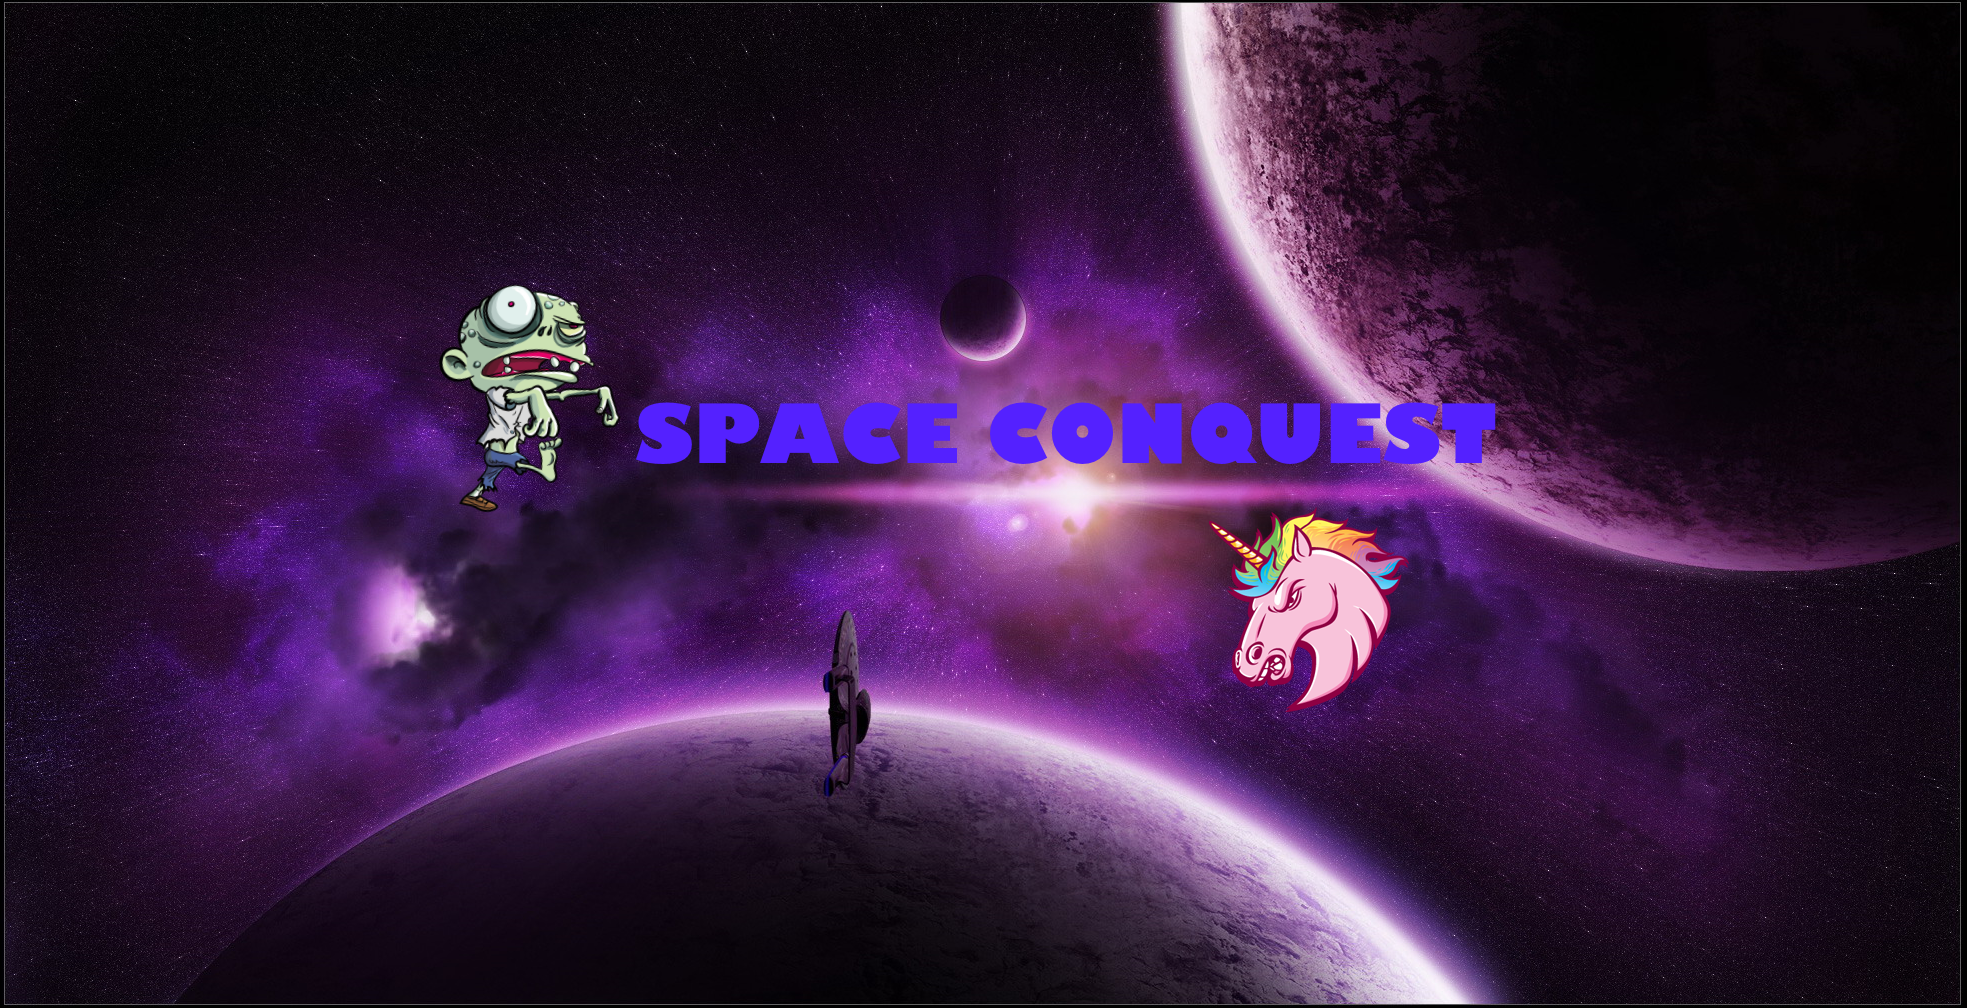
\includegraphics[scale=0.30]{Images/fondMenu.png}\\[2cm]
			\begin{center}
			\begin{Large}
				Baptiste Prunot\\
				Amaury Sauvage\\
				Raphael Pinto\\
				Hugo Ouertani\\
				Cyril Vandenbossche\\
				\end{Large}\\[2cm]
				
				
					\begin{flushright}
					\today
					\end{flushright}
					
				
				
				
			
			\end{center}
		\end{center}
		
	\end{titlepage}	
	
	\setcounter{tocdepth}{4}
	\tableofcontents
	
	\begin{center}
	\\[5cm]
	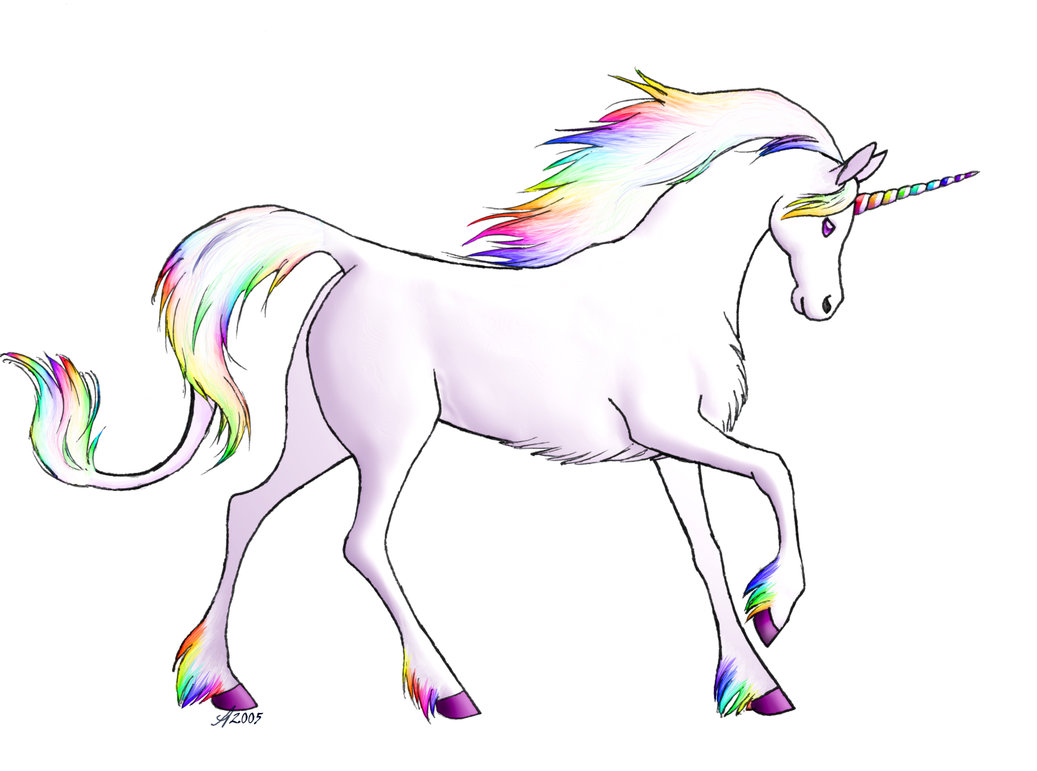
\includegraphics[scale=1]{Images/Licornes.jpg}
	\end{center}
	
	
	\chapter*{\textcolor{Fuchsia}{Génération des graphes et mode manuel}}
		\section*{\textcolor{Plum}{Génération des graphes}}
			
			\paragraph{\textcolor{purple}{Graphe de la carte}}
			Le graphe de la carte est la base sur laquelle vont \^etre g\'en\'er\'es le graphe des zombies, et celui des licornes.
			
			le graphe a la particularit\'e de repr\'esenter une carte avec des cases hexagonales. De ce fait, sa g\'en\'eration a entrain\'e quelques particularit\'es.
			
			Pour expliquer la methode utilis\'ee pour g\'en\'erer le graphe nous nous appuierons sur l'exemple d'une carte de taille 2.
			
			\begin{center}
				
					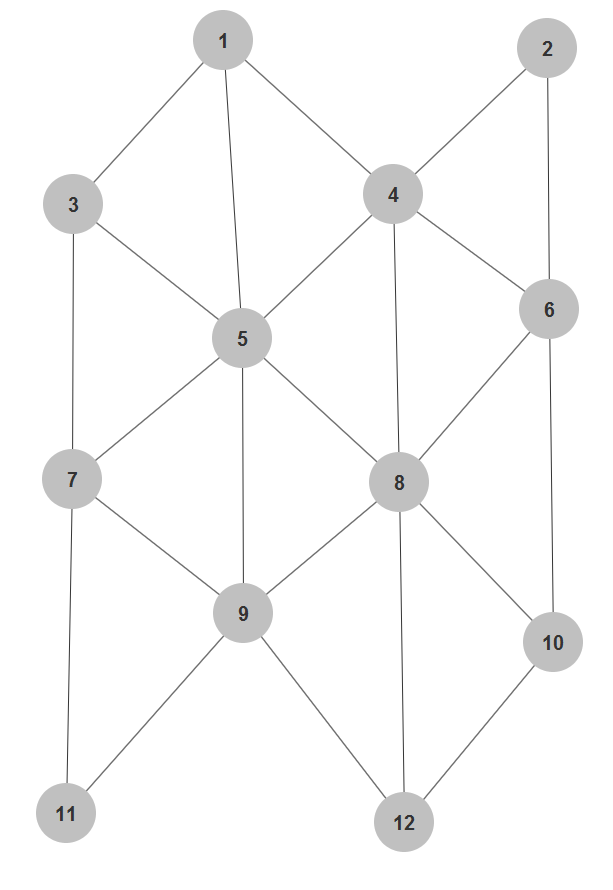
\includegraphics[scale=0.30]{Images/Graphe.png}
			
			\end{center}
			
			Si nous choisissons le sommet 1, nous remarquons qu'il est li\'e aux sommets suivants :
			
			\begin{itemize}
			
			
				\item le sommet 3 ce qui correspond à sommet+2 soit :
				
				
			
				$sommet+tailleGraphe$
				
				\item le sommet 5 ce qui correspond à sommet+4 soit :
				
				
				
				$sommet+tailleGraphe\times2$
				
				\item le sommet 4 ce qui correspond à sommet+3 soit : 
				
				
				
				$sommet+tailleGraphe+1$
				
			\end{itemize}
			
			On pourrait donc conclure que pour générer le graphe il suffirait de lier chaque sommet avec les observations faites ci-dessus. Cependant, bien que lier un sommet à son $sommet+taille\times2$ soit toujours vrai, les deux autres liaisons ne le sont pas forcément. ainsi on distingue deux cas :
			
			
			\begin{itemize}
			
			
				\item les lignes paires
				\item les lignes impaires
				\end{itemize}
				
			Lorsque la ligne est paire, un sommet est lié à trois sommets :
				
				\begin{itemize}
					\item $sommet+taille\times2$
					\item $sommet+taille$
					\item $sommet+taille-1$
				\end{itemize}
				
			En revanche lorsque la ligne est impaire, les liaisons sont définies de cette manière : 
				
				\begin{itemize}
					\item $sommet+taille\times2$
					\item $sommet+taille$
					\item $sommet+taille+1$
					\end{itemize}
					
			Ces observations aboutissent au code java suivant : 
			\\
			\begin{verbatim}
				public Graphe setGraphe(int taille) {
        Graphe graphe = new Graphe(taille);
        int nbSommet = graphe.getNbSommet();
        int n = this.taille;
        for (int i = 1; i <= nbSommet; i++) { 
            for (int j = 1; j <= n; j++) { 
                int position = j + (n * i) - n;
                if (position + n * 2 <= nbSommet) { 
                    graphe.ajouterArc(position, position + n * 2, 1);

                }
                if (position + n <= nbSommet) {
                    graphe.ajouterArc(position, position + n, 1);
                }

                if (i % 2 != 0) {    
                    if ((position + n + 1 <= nbSommet) && (j < n)) { 
                        graphe.ajouterArc(position, position + n + 1, 1);
                    }
                } else if (position + n - 1 <= nbSommet && (j > 1 && j <= n)) {
                    graphe.ajouterArc(position, position + n - 1, 1);
                }
            }
        }
        return graphe;
    }
			\end{verbatim}
			
			Un graphe de taille 2 généré par cette méthode donne la matrice d'adjacence suivante : 
			\\
			\begin{center}
			\setcounter{MaxMatrixCols}{13}
$					\begin{pmatrix}
			0&0&1&1&1&0&0&0&0&0&0&0\\
			0&0&0&1&0&1&0&0&0&0&0&0\\
			1&0&0&0&1&0&1&0&0&0&0&0\\
			1&1&0&0&1&1&0&1&0&0&0&0\\
			1&0&1&1&0&0&1&1&1&0&0&0\\
			0&1&0&1&0&0&0&1&0&1&0&0\\
			0&0&1&0&1&0&0&0&1&0&1&0\\
			0&0&0&1&1&1&0&0&1&1&0&1\\
			0&0&0&0&1&0&1&1&0&0&1&1\\
			0&0&0&0&0&1&0&1&0&0&0&1\\
			0&0&0&0&0&0&1&0&1&0&0&0\\
			0&0&0&0&0&0&0&1&1&1&0&0		
				\end{pmatrix}$
			\end{center}\\								
			

			
			\paragraph{\textcolor{purple}{Graphe des zombies}}
				
				Le graphe des zombies est similaire à celui de la carte, a une particularité prêt : il doit inclure le soleil, et traduire le fait qu'on ne peut pas aller dans le soleil. Dans la mesure ou chaque  $1$ de la matrice d'adjacence représente une liaison entre deux sommets du graphe, la solution envisagée a été de changer tous les $1$ en $0$ dans la colonne et la ligne correspondant au sommet qui contient le soleil.
				
				Pour ce faire, il a été décidé de rajouter une variable soleil contenant les coordonnées du soleil dans la classe carte, et une nouvelle méthode dans cette même classe pour calculer le numéro d'un sommet en fonction de ses coordonnées.
				
				Pour un sommet aux coordonnées $(x,y)$, la formule permettant de trouver le numéro est la suivante :
				
				\begin{center}
				 $ y+(x\times taille\_du\_graphe) - taille\_du\_graphe$			
				 \end{center}
	
				 Pour modéliser le soleil, il suffit donc de calculer le numéro de sommet du soleil avec la formule ci dessus, et de parcourir la matrice d'adjacence pour mettre une ligne de $0$ et une colonne de $0$ au numéro de ligne et de colonne correspondant au numéro de sommet contenant le soleil. Représenter le soleil de cette manière sur le graphe implique qu'il n'est pas possible d'aller sur le soleil, mais également qu'on ne peut aller nulle part de puis le soleil.
				 
				 Ce raisonnement aboutit à l'algorithme ci dessous :\\
				 
				 \begin{verbatim}
				 public void setGrapheZombie() {
        this.grapheZombie = this.graphe.clone();
        if (this.soleil != null) {
            int _soleil = this.position(this.soleil.getX(), this.soleil.getY());
            isolerSommet(_soleil, this.grapheZombie);

        }

    }
				\end{verbatim}
				
				la matrice d'adjacence résultante est la suivante. On remarquera que la colonne 6 et la ligne 6 sont une suite de 0, ce qui signifie que le soleil a été placé sur le sommet 6.\\
				\begin{center}
				\setcounter{MaxMatrixCols}{13}
				$\begin{pmatrix}
			0&0&1&1&1&0&0&0&0&0&0&0&\\
			0&0&0&1&0&0&0&0&0&0&0&0&\\
			1&0&0&0&1&0&1&0&0&0&0&0&\\
			1&1&0&0&1&0&0&1&0&0&0&0&\\
			1&0&1&1&0&0&1&1&1&0&0&0&\\
			0&0&0&0&0&0&0&0&0&0&0&0&\\
			0&0&1&0&1&0&0&0&1&0&1&0&\\
			0&0&0&1&1&0&0&0&1&1&0&1&\\
			0&0&0&0&1&0&1&1&0&0&1&1&\\
			0&0&0&0&0&0&0&1&0&0&0&1&\\
			0&0&0&0&0&0&1&0&1&0&0&0&\\
			0&0&0&0&0&0&0&1&1&1&0&0&
				\end{pmatrix}$	
				\end{center}
											  
				
			
			\paragraph{\textcolor{purple}{Graphe des licornes}}
			
			Une fois n'est pas coutume, le graphe des licornes est presque identique au graphe de la carte, et par extension au graphe des zombies, mais il doit traduire une contrainte supplémentaire : si les licornes veulent traverser une case contenant un champs d'astéroïdes, elles doivent dépenser deux points d'action.
			
			La manière de représenter cette contrainte a été traitée de manière très similaire à celle utilisée pour modéliser le soleil. En l'occurence, un tableau contenant les coordonnées de tous les astéroides placés a été créé. Lorsque le graphe des licornes est généré, le tableau est parcouru, et on calcule le numéro de sommet de chacun des astéroides. pour chaque numéro de ligne dans la matrice d'adjacence correspondant au sommet des astéroides, on remplace les $1$ par des $2$, ce qui indique que pour aller sur une case contenant un astéroïde, il faudra deux points d'action. en revanche, depuis une case contenant un astéroïde, aller vers une case vide ne coûtera qu'un point d'action.
			
			L'algorithme permettant de générer ce graphe est le suivant :\\
			\begin{verbatim}
			public void setGrapheLicornes() {
        this.grapheLicornes = this.grapheZombie.clone();
        if (this.asteroides != null) {
            for (int i = 0; i < this.asteroides.size(); i++) {
                //On boucle de manière à accéder à tous les asteroides.
                //pour chaque boucle, la position de l'astéroide est calculée
                int _asteroide = this.position(this.asteroides.get(i).getX(), this.asteroides.get(i).getY());
                //le graphe est parcouru ligne par ligne, et tous les 1 sont changés par des deux
                for (int j = 1; j <= this.taille * 3 * this.taille; j++) {
                    if (this.grapheLicornes.getMatrice(_asteroide, j) == 1) {
                        this.grapheLicornes.modifierMatrice(_asteroide, j, 2);
                    }
                }

            }
        }

    }
			\end{verbatim}
			
			La matrice d'adjacence produite par cette méthode est la suivante. On remarque que les lignes 3 et 4 comporte des $2$ et aucun $1$, des astéroides sont donc placés sur les cases 3 et 4.
			\setcounter{MaxMatrixCols}{13}
			\\
			\begin{center}
			$\begin{pmatrix}
			0&0&1&1&1&0&0&0&0&0&0&0&\\
			0&0&0&1&0&0&0&0&0&0&0&0&\\
			2&0&0&0&2&0&2&0&0&0&0&0&\\
			2&2&0&0&2&0&0&2&0&0&0&0&\\
			1&0&1&1&0&0&1&1&1&0&0&0&\\
			0&0&0&0&0&0&0&0&0&0&0&0&\\
			0&0&1&0&1&0&0&0&1&0&1&0&\\
			0&0&0&1&1&0&0&0&1&1&0&1&\\
			0&0&0&0&1&0&1&1&0&0&1&1&\\
			0&0&0&0&0&0&0&1&0&0&0&1&\\
			0&0&0&0&0&0&1&0&1&0&0&0&\\
			0&0&0&0&0&0&0&1&1&1&0&0&
			\end{pmatrix}$	
			\end{center}
			
		\section*{\textcolor{Plum}{Mode Manuel}}
			      \paragraph{\textcolor{purple}{Effacer la coloration}} 
    Pour effacer la coloration de la case, il suffit de colorier toutes les cases en blanc. 
    A cet effet, on réalise une boucle parcourant toutes les lignes  et une autre parcourant toutes les colonnes. A chaque passage de la boucle on crée un nouveau couple qui correspond à une case que l'on colorie en blanc. %la remarque sur le fait qu'il y a 3x plus de lignes que de colonne est pour moi inutile (on peut en débattre ^^)      
       
      Nous pouvons observer le résultat de cette fonction avec l'image ci-dessous, ici à titre d'exemple la carte a été coloriée en rouge.
       
      \begin{center}  
          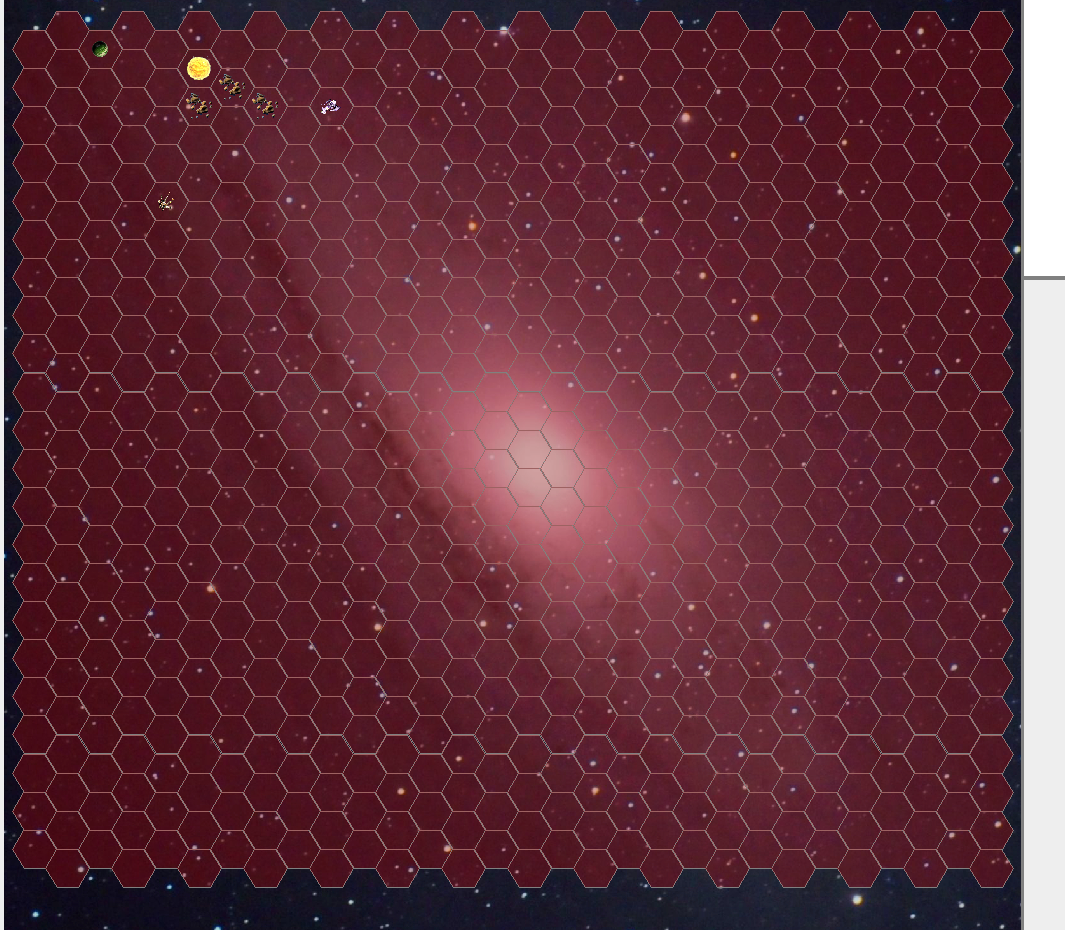
\includegraphics[scale=0.30]{Images/effaceColoration.png}
      \end{center} 
       
       
      \paragraph{\textcolor{purple} {Couleurs et distances}} 
      Ici le but est de colorier les cases ou le joueur peut se déplacer. 
      Pour cela on va  se servir de l'algorithme de Dijkstra, qui va calculer la distance minimum pour aller à chacun des sommets depuis la case du vaisseau du joueur. On va ensuite colorier les cases de distance 1 en vert et les cases de distances 2 en jaune.
       
      
			\paragraph{\textcolor{purple}{Mise en place de la coloration}}
			
			
			Pour que les cases sur lesquelles le joueur peut se déplacer s'affiche avec la couleur adéquat : 
			\begin{itemize}
				\item Vert pour une case nécessitant un point d'action
				\item Jaune pour une case nécessitant deux points d'action
			\end{itemize}
			il suffit de lire le tableau des distances généré par l'algorithme de Dijkstra. Chaque indice correspond à un sommet, par conséquent il faut colorier chaque sommet en fonction de sa valeur associée dans le tableau des distances. Ainsi, tous les sommets à 1 de distance seront coloriés en vert, et tous les sommets à 2 de distance seront coloriés en Jaune.\\[2cm]
			\begin{center} 
      
          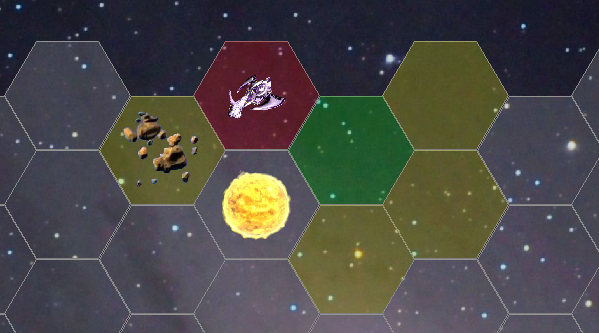
\includegraphics[scale=0.75]{Images/Coloration.png} 
     
      \end{center}
      
      \paragraph{\textcolor{purple}{Vérifier la validité d'un déplacement}}
      Pour limiter le déplacement du joueur aux cases coloriées lors de la sélection de son vaisseau, il faut vérifier que la seconde case qu'il choisi (la première étant le vaisseau) est à une distance de 1, ou de 2.
      Pour répondre à cette contrainte, le problème a été inversé. Lors de la sélection de la deuxième case, on ne vérifie pas que la nouvelle case est à une distance de 1 ou 2, mais on vérifie que le vaisseau est à une distance de 1 ou 2 de la case sélectionnée. Cette manière de procéder a été choisie pour exploiter la variable \emph{caseSelectionee} de la classe carte, et pour ne pas modifier de manière trop profonde la méthode \emph{selectionCase}.
      
      \paragraph{\textcolor{purple}{Implémentation de l'algorithme de Dijkstra}}
      La réalisation du projet de graphe repose en grande partie sur l'algorithme de Dijsktra, il est par conséquent nécessaire de donner quelques détails sur son implémentation.
       
      Le fonctionnement de l'algorithme repose sur l'utilisation de trois tableaux. Il a été décidé d'utiliser des ArrayLists, qui ont l'avantage d'avoir une limite dynamique. Un troisième tableau a été ajouté, il contient le numéro de tous les sommets, son utilité s'est limité aux tests d'exécution de l'algorithme.
      
      Lors de l'initialisation des tableaux, l'indice 0 est rempli avec une valeur fictive ($+\infty$ pour le tableau des distances, True pour le tableau de booléen, -1 pour les antécédents). Cela a pour avantage de pouvoir faire correspondre l'indice de chaque tableau avec un numéro de sommet. Les valeurs à l'indice 0 ont été choisie pour ne pas gêner le déroulement de l'algorithme. Représenter $+\infty$ s'est traduit par la création d'une fonction \emph{infini} qui renvoie la somme de tous les poids des arêtes+1.
      
      Pour déterminer si tous les sommets ont été traité au cours de l'exécution de l'algorithme, une fonction \emph{listeTerminee} a été créée. Elle lit le tableau de booléen et renvoie false si un élément dans ce tableau est à false.
       
		A chaque boucle de l'algorithme, il convient de connaitre le sommet non traité comportant la distance la plus courte. Une méthode a donc été rédiger pour renvoyer le sommet comportant la distance la plus courte. La méthode parcourt le tableau des distances, et récupère l'indice avec la plus faible valeur parmi les sommets non traités.	
			
			

	\chapter*{\textcolor{Fuchsia}{Mode automatique}}
		\section*{\textcolor{Plum}{Les races de base}}
			\paragraph{\textcolor{purple}{Mouvement des licornes}}
			Le principe est ici de calculer un chemin gr\^ace \`a l'algorithme de dijkstra. Pour ce faire, on utilise une m\'ethode r\'eccurcive qui va lire le tableau des ant\'ec\'edents. Initialementm l'algorithme impl\'ement\'e calcule le chemin le plus court pour parcourir tout le graphe (soit du premier au dernier sommet). Pour qu'un chemin soit g\'en\'er\'e d'un point de d\'epart jusqu'a un point d'arriv\'ee, il suffit de lire le tableau des ant\'ec\'edents jusqu'a trouver le sommet sans ant\'ec\'edent (Le sommet sans ant\'ec\'edent a, dans les faits, -1 comme ant\'ec\'edent). une fois le chemin trouv\'e il est stock\'e dans un tableau, que les licornes vont lire \`a chaque tour gr\^ace \`a un compteur.
			\paragraph{\textcolor{purple}{Mouvement des zombies}}
			
			La solution retenue pour que les zombies ce dirigent vers les licornes en passant par le plus court chemin a \'et\'e de calculer le chemin le plus court \`a chaque tour gr\^ace \`a l'algorithme de Dijkstra. Une autre solution avait un temps \'et\'e envisag\'ee, celle d'utiliser l'algorithme de floyd Warshall, pour stocker tous les chemins les plus courts entre tous les couples de sommets du graphe des zombies. N\'enmoins, le nombre de chemin a calculer devenait rapidement cons\'equent, et il fallait jusqu'\`a une minute pour voir apparaitre la carte du jeu. Pour cette raison il a sembl\'e plus judicieux de calculer le chemin a chaque tour.
			
	\section*{\textcolor{Plum}{Les shadocks et les gibis}}			
			\paragraph{\textcolor{purple}{Les shadocks}}
			Le trajet des shadocks se calcule en deux temps :
				
			\begin{itemize}
				\item On calcule le plus court chemin a partir de la plan\'ete shadock, et on stocke tous les sommet a 3 de distances ou moins dans un arraylist.
				\item A chaque tour des shadocks, on calcule le chemin le plus court depuis leur position. il suffit ensuite de d\'eplacer le vaisseau shadock sur une a 1 de distance de leur vaisseau, et a maximum 3 de distance de leur plan\`te (la comparaison est possible gr\^ace \`a l'ArrayList \'evoqu\'e pr\'ec\'edemment.
			\end{itemize}

			\paragraph{\textcolor{purple}{Optimisation des gibis}}
			Une façon de ré aliser cette optimisation est de rep\'erer toutes les cases sur lesquelles le vaisseau shadock peut se d\'eplacer durant un tour donn\'e, puis d'interdire ces sommets aux licornes.
			Dans un premier temps on va servir de la fonction "AntiShadock" permettant de stocker à partir de l'algorithme de dijkstra tous les sommets de distance inf\'erieure ou \'egale \`a 2.
			Puis dans un second temps on peut grâce à la fonction plus court chemin que l'on surcharge d'un paramètre ArrayList, isoler les sommets de ce fait il sera impossible pour les licorne d'y aller.
			\paragraph{\textcolor{purple}{Navigation suicidaire}}
			Le principe ici est de faire en sorte que le vaisseau licorne ne se jette pas sur le vaisseau des zombies.
			
			Pour ce faire il suffit de reprendre le principe d'isolation du sommet su soleil, ce qui conduit à traiter le vaisseau des zombies comme un "soleil mouvant". Il n'y a néanmoins pas de modification de graphes, il suffit simplement de marquer à l'initialisation de l'algorithme de Dijkstra le sommet sur lequel est positionné le vaisseau des zombie comme déjà traité. Le résultat est que la distance pour aller à ce sommet restera à $+\infty$, c'est à dire inaccessible pour les licornes quelque soit le mode de jeu.
			\begin{center}  
          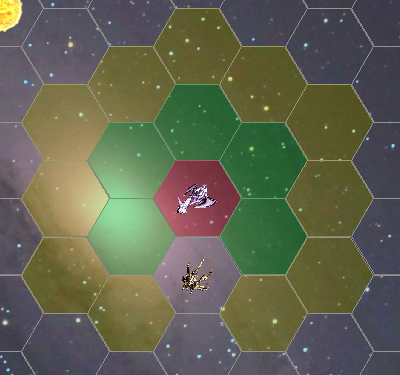
\includegraphics[scale=0.30]{Images/isoleZombie.png}
      		\end{center} 
      		
      		L'algorithme aboutit au résultat ci-dessus.
      
			\paragraph{\textcolor{purple}{Coloniser plusieurs planètes}}
			La possibilité pour les licornes de coloniser plusieurs planètes, et notamment de se diriger vers la plus proche, a été rendu possible grâce a un ArrayList, ainsi que le tableau des distances, et celui des antécédents donnés par l'exécution de l'algorithme de Dijkstra.
			
			En début de partie, chaque fois qu'une planète est ajoutée sur la carte, ces coordonnées sont stockées dans un ArrayList. A chaque tour des licornes, l'algorithme de Dijkstra est exécuté, et les coordonnées des planètes vont être converti en numéro de sommet. Grâce à ces numéros, il suffira de lire pour chaque sommet la distance la plus courte, et construire un chemin vers la planète la plus proche.
			
			Une fois que la planète est atteinte, elle est effacée de l'ArrayList, ce qui permet au vaisseau des licornes de se diriger vers la planète suivante et de ne pas rester sur la planète atteinte.\\[3cm]
			\begin{center}
			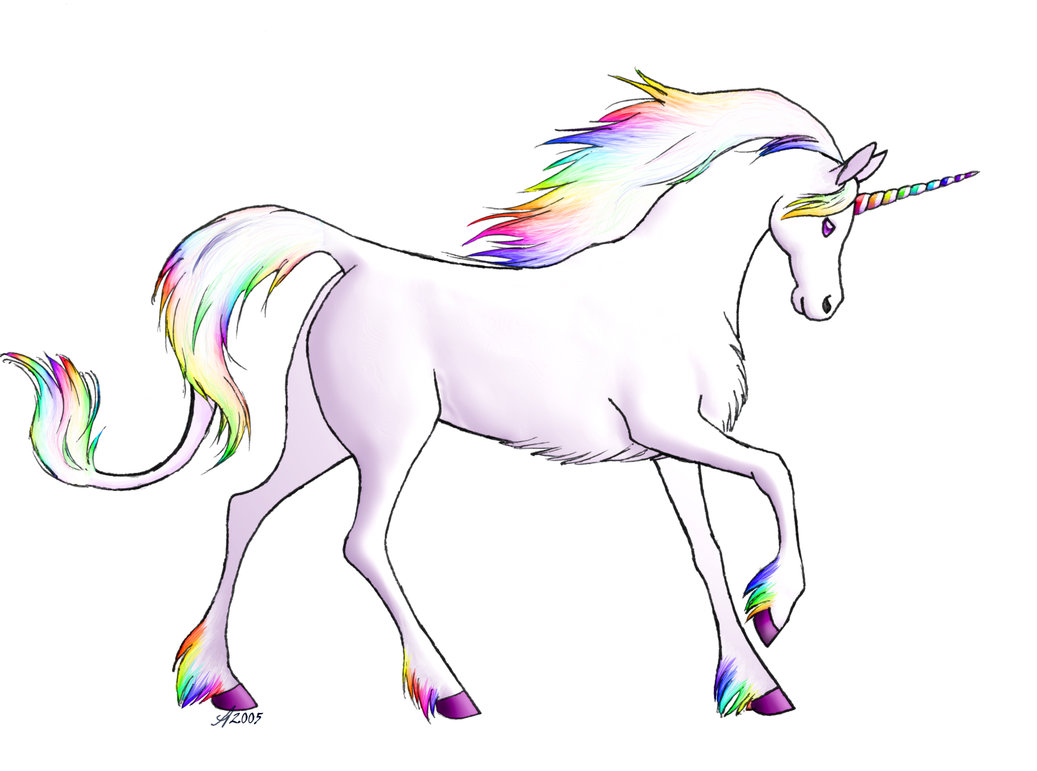
\includegraphics[scale=1]{Images/Licornes.jpg}
			\end{center}
			

\end{document}
